% Biên dịch: xelatex results.tex (chạy 2 lần để cập nhật mục lục)
\documentclass[11pt,a4paper]{article}
\usepackage{fontspec}
\setmainfont{Times New Roman}
\setsansfont{Arial}
\setmonofont{Consolas}
\usepackage[a4paper,margin=2.2cm]{geometry}
\usepackage{amsmath,amssymb}
\usepackage{graphicx}
\usepackage{booktabs,tabularx,array,multirow}
\usepackage{xcolor}
\usepackage{enumitem}
\usepackage{caption}
\usepackage{float}
\usepackage[colorlinks=true,linkcolor=blue!50!black,citecolor=blue!50!black,urlcolor=blue!50!black]{hyperref}
\setlist{itemsep=2pt,topsep=4pt}
\emergencystretch=3em
\renewcommand{\arraystretch}{1.18}
\newcolumntype{Y}{>{\raggedright\arraybackslash}X}
\captionsetup{font=small,labelfont=bf}
\newcommand{\W}{W_{\text{float}}}
\newcommand{\dW}{\Delta W_{\text{float}}}
\definecolor{okc}{HTML}{1D7A4F}\definecolor{noc}{HTML}{B23A2E}\definecolor{partc}{HTML}{9A6A00}
\newcommand{\ok}{\textcolor{okc}{\textbf{Được ủng hộ}}}
\newcommand{\no}{\textcolor{noc}{\textbf{Không được ủng hộ}}}
\newcommand{\partly}{\textcolor{partc}{\textbf{Ủng hộ một phần}}}
\newcommand{\interp}{\par\smallskip\noindent\textbf{Diễn giải.}~}

\title{\textbf{Tổng hợp kết quả thực nghiệm}\\[3pt]
\large Floater do sai lệch trắc quang giữa các ảnh trong 3D Gaussian Splatting}
\author{Nhóm FaithfulRecon --- Trường Đại học Bách khoa, ĐHQG-HCM\\
Tài liệu nội bộ cho thành viên nhóm}
\date{16/11/2026}

\begin{document}
\maketitle

\begin{abstract}
\noindent Tài liệu tổng hợp toàn bộ thí nghiệm đã thực hiện (pha 1: 336 checkpoint trên 3 scan DTU với pipeline nghiên cứu; pha 2 (v2): khoảng 267 lượt huấn luyện, gồm 135 lượt 3DGS chuẩn trên 15 scan DTU và các thí nghiệm khoá cơ chế), kèm số liệu, diễn giải và trạng thái từng giả thuyết. Kết quả chính: (1) sai lệch trắc quang theo từng ảnh làm tăng tỉ lệ đóng góp kết xuất của Gaussian ngoài bề mặt ở mọi cấu hình đã thử, kể cả 3DGS chuẩn trên 15/15 scan; (2) yếu tố quyết định là sự khác nhau của phép biến đổi giữa các camera cùng quan sát một vùng, và cách gán nhiễu lên camera thay đổi độ lớn tác động tới khoảng 2 lần khi giữ nguyên tập tham số; (3) dung lượng biểu diễn màu không phải nút thắt: SH bậc 3 và affine học bằng gradient giữ phần lớn floater, trong khi căn chỉnh dạng đóng có ràng buộc gauge (GC-ILA) xoá gần hết hiệu ứng, tương đương bù chính xác, khi khởi tạo tốt; (4) sai lệch rò vào hình học từ những vòng lặp đầu, qua độ mờ của các Gaussian có sẵn; giả thuyết ``bù học chậm hơn mật độ hoá'' không được ủng hộ; (5) không có tương tác nhất quán giữa số góc nhìn và mức sai lệch. Các giới hạn chính: chỉ dùng DTU và nhiễu ISP tổng hợp; một số thí nghiệm cơ chế mới có 2 scan.
\end{abstract}

\tableofcontents
\newpage

%=====================================================================
\section{Mục tiêu và giả thuyết ban đầu}
Câu hỏi nghiên cứu: \emph{độ phủ đa góc nhìn hạn chế ($N$) và sai lệch trắc quang giữa các góc nhìn ($S$) tác động riêng rẽ và đồng thời như thế nào đến sự hình thành Gaussian ngoài bề mặt trong 3DGS?} Các dự đoán ban đầu:
\begin{itemize}
  \item[\textbf{P1.}] Với $N$ cố định, chỉ số floater tăng theo $S$.
  \item[\textbf{P2.}] Mức tăng trong P1 lớn hơn khi $N$ nhỏ hơn (tương tác).
  \item[\textbf{P3.}] Floater do sai lệch trắc quang nằm phía trước bề mặt theo hướng nhìn.
  \item[\textbf{P4.}] Cải thiện chỉ số ảnh nhờ mô-đun bù ngoại hình không nhất thiết đi kèm cải thiện hình học.
\end{itemize}
Trong quá trình thực nghiệm, nhóm bổ sung các giả thuyết về cơ chế (Mục~\ref{sec:status}).

%=====================================================================
\section{Giao thức chung}
\label{sec:protocol}
\begin{itemize}
  \item \textbf{Dữ liệu.} DTU (định dạng IDR/NeuS), ảnh $400\times300$, nền trắng ngoài mặt nạ vật thể. Cảnh chuẩn hoá vào hình cầu bán kính xấp xỉ 1. $N$ view huấn luyện chọn bằng farthest-point sampling trên tâm camera (tập lồng nhau theo $N$).
  \item \textbf{Nhiễu trắc quang} (chỉ ảnh huấn luyện, trong mặt nạ):
  \begin{gather*} I'_k=\operatorname{clip}(g_k\,\mathbf{w}_k\odot I_k)^{\gamma_k},\\
  g_k=2^{e_k},\ e_k\sim\mathcal U(-s,s);\quad \mathbf{w}_k=e^{\mathbf u_k},\ \mathbf u_k\sim\mathcal U(-b,b)^3;\quad \gamma_k=e^{v_k},\ v_k\sim\mathcal U(-\gamma,\gamma). \end{gather*}
  Mức mild $(s,b,\gamma)=(0.5,0.05,0.10)$, strong $(1.0,0.15,0.20)$, seed nhiễu 0 trừ khi ghi khác.
  \item \textbf{Chỉ số chính.} $d_i$ là khoảng cách từ tâm Gaussian $i$ tới bề mặt tham chiếu STL (đơn vị chuẩn hoá).
  \[ \W(\tau)=\frac{\sum_{k\in\mathcal T}\sum_{\mathbf p}\sum_{i:d_i>\tau}w_{ik}(\mathbf p)}{\sum_{k\in\mathcal T}\sum_{\mathbf p}\sum_i w_{ik}(\mathbf p)},\quad \tau=0.1, \]
  với $w_{ik}(\mathbf p)$ là trọng số trộn chính xác (renderer PyTorch) trên 16 view kiểm định $\mathcal T$.
  \item \textbf{Đánh giá cuối (áp dụng cho mọi số liệu trong tài liệu, trừ khi ghi khác).} Bề mặt tham chiếu \emph{lọc chặt}: chỉ giữ điểm STL nằm trong mặt nạ ở $\ge 80\%$ số view mà điểm chiếu vào (giữ 69\%, 43\%, 30\% số điểm của scan24, scan63, scan83). 16 view kiểm định chọn ngoài 16 camera FPS đầu tiên, chung cho mọi $N\le16$. Mọi checkpoint được đánh giá bằng renderer PyTorch, kể cả khi huấn luyện bằng gsplat.
  \item \textbf{So sánh theo cặp.} $\dW=\W(\text{mức nhiễu})-\W(\text{none})$ cùng scan, seed, $N$ và cùng cấu hình huấn luyện. Với biến thể chỉ khác ở nhiễu (nhiễu toàn cục, theo pixel, oracle, không clip, hoán vị), mức none là của cấu hình huấn luyện tương ứng. ``up'' là số cặp tăng trên tổng số cặp.
  \item \textbf{Hai pipeline.}
  \begin{itemize}
    \item \emph{Pipeline nghiên cứu} (pha 1 và phần lớn v2): renderer PyTorch, màu RGB (SH bậc 0), khởi tạo 10\,000 điểm ngẫu nhiên trong $[-1,1]^3$, 7000 vòng, mật độ hoá 300--3500, 3 seed (5 seed cho cấu hình gốc $N=8$ của scan63, scan83).
    \item \emph{3DGS chuẩn} (T2, v2): gsplat, SH bậc 3, khởi tạo từ điểm triangulate trên ảnh huấn luyện sạch với pose đã biết (SIFT, kiểm tra epipolar, DLT), 10\,000 vòng, mật độ hoá 500--5000, 15 scan chuẩn của DTU.
  \end{itemize}
\end{itemize}

\begin{table}[H]
\centering\small
\caption{Danh mục thí nghiệm.}
\begin{tabularx}{\textwidth}{@{}l Y l l@{}}
\toprule
ID & Câu hỏi & Pipeline & Mục \\
\midrule
E0 & Độ nhạy theo $\tau$, phân rã đóng góp floater & nghiên cứu & \ref{sec:p1} \\
P1 & Floater tăng theo $S$ ($N=8$, 3 scan) & nghiên cứu & \ref{sec:p1} \\
E2b, E2c, E6 & Số view quan sát floater; Gaussian lớn; giữ cắt kích thước & nghiên cứu & \ref{sec:p1} \\
E5 & SH bậc 3 & nghiên cứu & \ref{sec:mech} \\
E1, E1b, E4b-$\gamma$ & Nhiễu theo pixel; cùng biến đổi cho mọi ảnh; nhiễu không $\gamma$ & nghiên cứu & \ref{sec:mech} \\
E4, E4b, E4c, M1 & Affine học (lr $10^{-3}$, $10^{-2}$); oracle; căn chỉnh dạng đóng & nghiên cứu & \ref{sec:comp} \\
E3, E3b & Lưới $N\times S$, $N\in\{4,6,8,12,16\}$ & nghiên cứu & \ref{sec:nxs} \\
E9 & Khởi tạo visual hull & nghiên cứu & \ref{sec:init} \\
E8, E11 & Cấu hình nhiễu khác; thêm seed & nghiên cứu & \ref{sec:p1} \\
E7 & Tín hiệu phát hiện floater & nghiên cứu & \ref{sec:e7} \\
T0 & Chỉ số xung đột $I_{\text{conflict}}$; $\W^\Sigma$ & không huấn luyện & \ref{sec:ea}, \ref{sec:wsig} \\
T2 & Go/no-go: 3DGS chuẩn, 15 scan & chuẩn & \ref{sec:t2} \\
E13 & Ngoại lệ oracle: clip, mặt nạ bão hoà & nghiên cứu & \ref{sec:e13} \\
M2 & GC-ILA (căn chỉnh dạng đóng có gauge) & nghiên cứu & \ref{sec:gc} \\
E12 & Thời điểm bù (warm-up), quỹ đạo $\W(t)$ & nghiên cứu, visual hull & \ref{sec:e12} \\
E-A & Hoán vị cách gán nhiễu lên camera & nghiên cứu & \ref{sec:ea} \\
\bottomrule
\end{tabularx}
\end{table}

%=====================================================================
\section{Kết quả pha 1 (pipeline nghiên cứu)}

\subsection{P1 và độ vững}
\label{sec:p1}
\begin{table}[H]
\centering\small
\caption{$\W(0.1)$ và $\dW$, $N=8$, cấu hình gốc. Số seed: 3 (scan24), 5 (scan63, scan83).}
\begin{tabular}{@{}lccccccc@{}}
\toprule
Scan & none & mild & strong & $\dW$ mild & $\dW$ strong & PSNR none & PSNR strong \\
\midrule
scan24 & 0.332 & 0.470 & 0.593 & $+0.137$ (3/3) & $+0.261$ (3/3) & 16.78 & 11.10 \\
scan63 & 0.262 & 0.359 & 0.467 & $+0.096$ (5/5) & $+0.204$ (5/5) & 24.24 & 19.41 \\
scan83 & 0.162 & 0.277 & 0.486 & $+0.115$ (5/5) & $+0.324$ (5/5) & 25.97 & 21.08 \\
\bottomrule
\end{tabular}
\end{table}
\begin{itemize}
  \item 26/26 cặp tăng; trung bình $+0.113$ (mild), $+0.263$ (strong).
  \item \textbf{E0 (đánh giá ban đầu).} $\W(\tau)$ và off$(\tau)$ tăng đơn điệu none $<$ mild $<$ strong với $\tau\in\{0.03,0.05,0.1,0.15\}$ trên cả 3 scan (24/24 so sánh). Ở mức strong, đóng góp kết xuất của floater tăng $\times2.1$--$\times5.1$, nhanh hơn số lượng floater ($\times1.7$--$\times2.1$), còn đóng góp của Gaussian gần bề mặt giảm ($\times0.64$--$\times0.89$): floater che bề mặt chứ không chỉ cộng thêm.
  \item \textbf{E2b.} Trên scan63, scan83, chỉ 1--27\% mức tăng đến từ floater được $\le2$ view quan sát; ở scan83 mức strong, floater được trung bình 4.1/8 view quan sát. Khoảng cách tới camera huấn luyện gần nhất chỉ giảm 4--8\%. Giả định ``floater riêng cho 1--2 view, sát camera'' không được ủng hộ.
  \item \textbf{E2c, E6.} Khoảng 7 Gaussian rất lớn chiếm 23--34\% mức tăng; giữ cắt kích thước tới hết huấn luyện vẫn giữ 91\% (scan63) và 106\% (scan83) mức tăng (đánh giá cuối). Floater bị loại được thay thế bởi Gaussian khác.
  \item \textbf{E8 (cấu hình nhiễu khác, cùng biên độ).} $\dW$ strong: $+0.109$, $+0.219$ (scan63); $+0.081$, $+0.269$ (scan83); 12/12 cặp tăng. Độ lớn thay đổi 3--4 lần theo cách tham số phân bố trên các ảnh, lớn hơn nhiều so với dao động giữa seed huấn luyện.
  \item \textbf{E11 (5 seed).} Mức none của cấu hình gốc dao động 0.251--0.276 (scan63), 0.137--0.186 (scan83). Với affine học, mức none trên scan83 dao động 0.120--0.405.
  \item \textbf{Bề mặt tham chiếu.} So với bề mặt cũ (lọc lỏng), $\W$ thay đổi $\le0.006$ trên scan24, scan63; trên scan83, mức none tăng 0.124 $\to$ 0.162. Chiều của mọi so sánh giữ nguyên.
\end{itemize}

\subsection{Cấu trúc nhiễu và biểu diễn màu}
\label{sec:mech}
\begin{figure}[H]
\centering
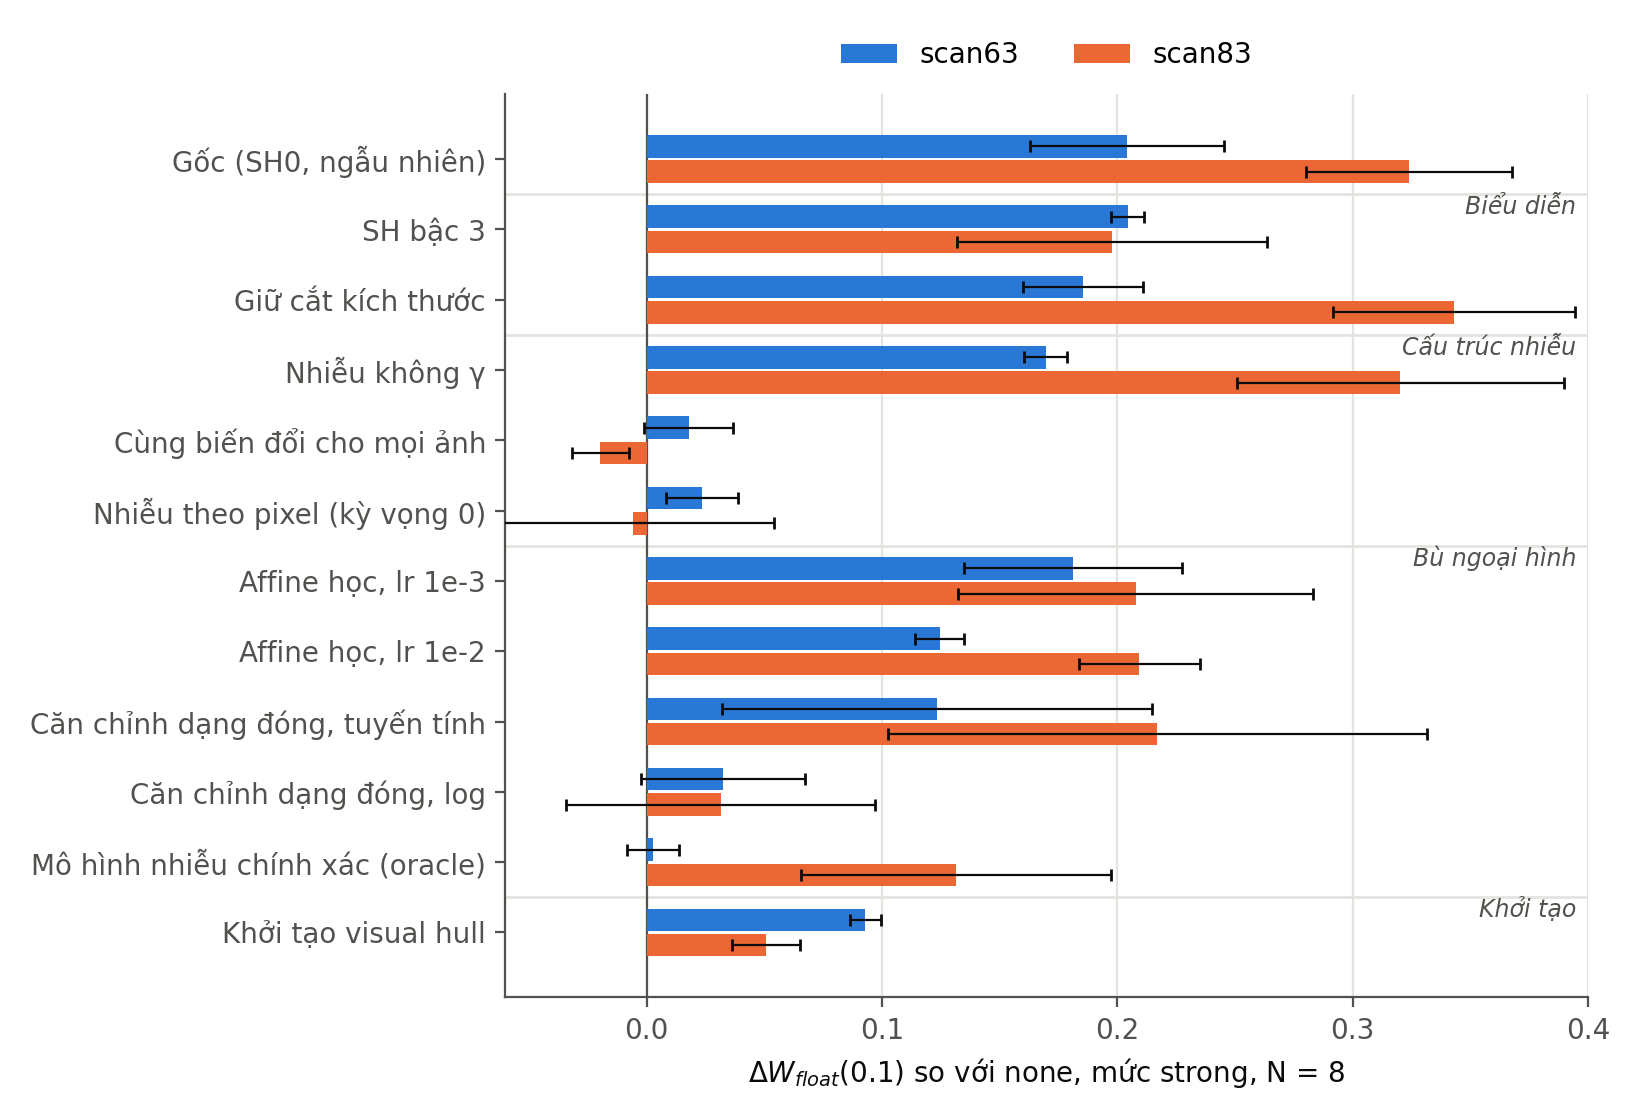
\includegraphics[width=0.88\textwidth]{figures/final_mechanism.png}
\caption{$\dW$ mức strong, $N=8$, mọi biến thể của pha 1. Thanh: trung bình theo seed; đoạn đen: độ lệch chuẩn.}
\label{fig:mech}
\end{figure}
\begin{table}[H]
\centering\small
\caption{$\dW$ (scan63 / scan83), $N=8$.}
\begin{tabular}{@{}lccl@{}}
\toprule
Biến thể & mild & strong & Tỉ lệ so với gốc (strong) \\
\midrule
Gốc (SH0) & $+0.096$ / $+0.115$ & $+0.204$ / $+0.324$ & 1 \\
SH bậc 3 (E5) & $+0.092$ / $+0.016$ & $+0.204$ / $+0.198$ & 1.00 / 0.61 \\
Giữ cắt kích thước (E6) & $+0.082$ / $+0.127$ & $+0.185$ / $+0.343$ & 0.91 / 1.06 \\
Nhiễu không $\gamma$ & -- & $+0.170$ / $+0.320$ & 0.83 / 0.99 \\
Cùng biến đổi cho mọi ảnh (E1b) & $+0.001$ / $+0.094$ & $+0.018$ / $-0.020$ & 0.09 / $-0.06$ \\
Nhiễu theo pixel, kỳ vọng 0 (E1) & $+0.003$ / $-0.014$ & $+0.024$ / $-0.006$ & 0.12 / $-0.02$ \\
\bottomrule
\end{tabular}
\end{table}
\interp Khi mọi ảnh cùng chịu một biến đổi (E1b), mỗi ảnh vẫn lệch so với ảnh gốc ít nhất bằng ảnh lệch nhất của nhiễu ISP và PSNR giảm (19.57 / 22.90 dB), nhưng hình học hầu như không đổi: mô hình hấp thụ biến đổi chung vào màu. Nhiễu theo pixel cùng độ lớn cũng không gây floater. Vậy yếu tố gây floater là \textbf{sự khác nhau của phép biến đổi giữa các ảnh}, không phải độ lệch so với ảnh gốc. Thành phần phi tuyến $\gamma$ không cần thiết. SH bậc 3 có thể biểu diễn màu phụ thuộc hướng nhìn nhưng vẫn giữ 61--100\% mức tăng. Ngoại lệ: E1b scan83 mức mild ($+0.094$, độ lệch chuẩn 0.156) do một seed.

\subsection{Bù ngoại hình (E4, E4b, E4c, M1)}
\label{sec:comp}
Mọi mô-đun bù chỉ áp lên ảnh kết xuất trong hàm mất mát; ảnh kiểm định kết xuất không qua mô-đun (PSNR trực tiếp). PSNR căn chỉnh: khớp một phép affine theo kênh giữa ảnh kết xuất và ảnh kiểm định trước khi tính PSNR.
\begin{table}[H]
\centering\small
\caption{Bù ngoại hình, $N=8$, khởi tạo ngẫu nhiên (scan63 / scan83).}
\begin{tabular}{@{}lcccc@{}}
\toprule
Biến thể & $\W$ none & $\dW$ strong & PSNR trực tiếp strong & PSNR căn chỉnh strong \\
\midrule
Gốc & 0.262 / 0.162 & $+0.204$ / $+0.324$ & 19.41 / 21.08 & 20.35 / 21.44 \\
Affine học, lr $10^{-3}$ & 0.257 / 0.251 & $+0.181$ / $+0.208$ & 20.37 / 21.10 & 20.94 / 21.36 \\
Affine học, nhiễu không $\gamma$ & -- & $+0.136$ / $+0.175$ & 20.42 / 21.18 & -- \\
Affine học, lr $10^{-2}$ & 0.251 / 0.256 & $+0.125$ / $+0.209$ & 21.24 / 22.16 & 21.62 / 22.47 \\
Căn chỉnh dạng đóng, tuyến tính & 0.262 / 0.571 & $+0.123$ / $+0.217$ & 10.49 / 9.88 & -- \\
Căn chỉnh dạng đóng, log (M1) & 0.311 / 0.193 & $+0.033$ / $+0.032$ & 12.33 / 12.71 & 18.94 / 17.48 \\
Oracle (biết chính xác nhiễu) & -- & $+0.003$ / $+0.132$ & 24.27 / 25.82 & 24.35 / 25.86 \\
\bottomrule
\end{tabular}
\end{table}
\interp (i) Affine học giữ 61--89\% mức tăng, kể cả khi nhiễu không có $\gamma$ (phép biến đổi thật nằm trọn trong lớp affine): thất bại không do sai lớp mô hình. (ii) Affine học tăng PSNR 0--2 dB nhưng giảm floater ít; M1 giảm floater mạnh nhưng mất màu tuyệt đối. Cải thiện ảnh và cải thiện hình học tách rời theo cả hai chiều (P4). (iii) PSNR căn chỉnh của M1 vẫn chỉ 17--19 dB: màu trôi không chỉ là một phép affine toàn cục, nên cần ràng buộc gauge (Mục~\ref{sec:gc}).

\subsection{Lưới $N\times S$ (E3, E3b)}
\label{sec:nxs}
\begin{figure}[H]
\centering
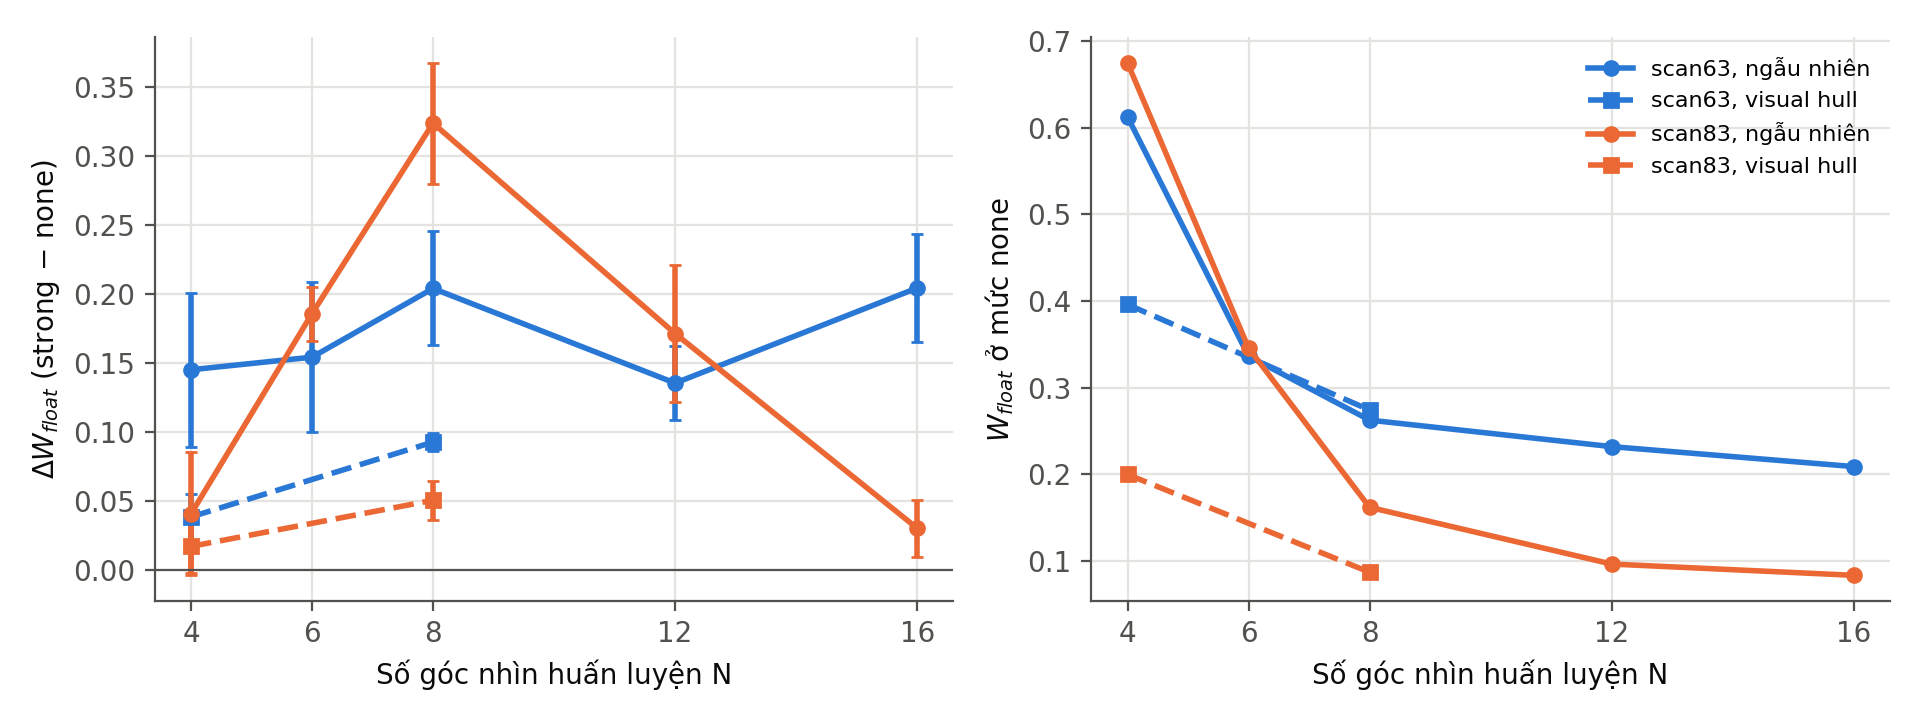
\includegraphics[width=\textwidth]{figures/final_nxs.png}
\caption{Trái: $\dW$ mức strong theo $N$. Phải: $\W$ mức none. Nét liền: khởi tạo ngẫu nhiên; nét đứt: visual hull.}
\end{figure}
\begin{table}[H]
\centering\small
\caption{$\dW$ theo $N$, khởi tạo ngẫu nhiên.}
\begin{tabular}{@{}llccccc@{}}
\toprule
Scan & Mức & $N=4$ & $N=6$ & $N=8$ & $N=12$ & $N=16$ \\
\midrule
scan63 & mild & $+0.023$ & $+0.048$ & $+0.096$ & $+0.041$ & $+0.081$ \\
scan63 & strong & $+0.145$ & $+0.154$ & $+0.204$ & $+0.136$ & $+0.205$ \\
scan83 & mild & $-0.041$ & $+0.098$ & $+0.115$ & $+0.037$ & $+0.015$ \\
scan83 & strong & $+0.041$ & $+0.186$ & $+0.324$ & $+0.172$ & $+0.030$ \\
\midrule
\multicolumn{2}{@{}l}{$\W$ none (63 / 83)} & 0.61 / 0.68 & 0.34 / 0.35 & 0.26 / 0.16 & 0.23 / 0.10 & 0.21 / 0.08 \\
\bottomrule
\end{tabular}
\end{table}
Hồi quy logit, hiệu ứng cố định theo scan, $S\in\{0,0.5,1\}$, khoảng tin cậy 95\% bằng bootstrap theo (scan, seed):
\begin{itemize}
  \item $N=4$--16 (102 lượt): $\hat\beta_N=-0.176\ [-0.226,-0.120]$, $\hat\beta_S=+0.771\ [+0.577,+1.004]$, $\hat\beta_{NS}=+0.009\ [-0.007,+0.023]$; tác động của $S$ trên thang logit 0.81 ($N=4$) đến 0.91 ($N=16$).
  \item $N\le8$ (66 lượt): $\hat\beta_{NS}=+0.209\ [+0.103,+0.308]$.
  \item Visual hull, $N\in\{4,8\}$: $\hat\beta_{NS}=+0.084\ [+0.067,+0.101]$.
\end{itemize}
\interp Tương tác dương ở $N\le8$ không kéo dài tới $N=16$; trên toàn khoảng, tác động của $S$ gần như không đổi trên thang logit. Hai scan có dạng khác nhau trên thang tuyệt đối. \textbf{P2 không được ủng hộ.} Ở $N=16$, mức strong vẫn tăng floater ở 6/6 cặp: tăng số view không tự loại bỏ tác động.

\subsection{Khởi tạo (E9)}
\label{sec:init}
\begin{table}[H]
\centering\small
\caption{Khởi tạo ngẫu nhiên và visual hull (10\,000 điểm trong visual hull của mặt nạ huấn luyện).}
\begin{tabular}{@{}llcccccc@{}}
\toprule
& & \multicolumn{2}{c}{$\W$ none} & \multicolumn{2}{c}{$\dW$ strong} & \multicolumn{2}{c}{PSNR none} \\
\cmidrule(lr){3-4}\cmidrule(lr){5-6}\cmidrule(lr){7-8}
Scan & $N$ & Ngẫu nhiên & Hull & Ngẫu nhiên & Hull & Ngẫu nhiên & Hull \\
\midrule
scan24 & 8 & 0.332 & 0.265 & $+0.261$ & $+0.153$ & 16.78 & 19.81 \\
scan63 & 4 & 0.612 & 0.396 & $+0.145$ & $+0.039$ & 14.17 & 17.58 \\
scan63 & 8 & 0.262 & 0.274 & $+0.204$ & $+0.093$ & 24.24 & 23.72 \\
scan83 & 4 & 0.675 & 0.200 & $+0.041$ & $+0.017$ & 16.42 & 19.48 \\
scan83 & 8 & 0.162 & 0.087 & $+0.324$ & $+0.051$ & 25.97 & 25.98 \\
\bottomrule
\end{tabular}
\end{table}
\interp Với visual hull, mức tăng còn 16--59\% nhưng vẫn dương ở mọi cặp $N=8$: P1 đúng với khởi tạo tốt. Khởi tạo ngẫu nhiên khuếch đại tác động 2--6 lần; số liệu pha 1 nên được hiểu là cận trên.

\subsection{Tín hiệu phát hiện floater (E7)}
\label{sec:e7}
\begin{table}[H]
\centering\small
\caption{AUROC có trọng số theo đóng góp trên view kiểm định; nhãn floater $d>0.1$; $N=8$, 3 mức $\times$ 3 seed. Giá trị $<0.5$: tín hiệu có chiều ngược.}
\begin{tabular}{@{}lccc@{}}
\toprule
Tín hiệu & scan63 & scan83 & scan63: none / mild / strong \\
\midrule
Bất đồng giữa hai seed & 0.84 & 0.89 & 0.81 / 0.83 / 0.87 \\
Kích thước lớn & 0.78 & 0.83 & 0.76 / 0.78 / 0.79 \\
$n_{\text{vis}}$ thấp & 0.57 & 0.25 & 0.65 / 0.59 / 0.48 \\
Độ mờ thấp & 0.33 & 0.33 & 0.32 / 0.35 / 0.33 \\
\bottomrule
\end{tabular}
\end{table}
\interp Bất đồng giữa hai mô hình là tín hiệu tốt nhất và không suy giảm khi $S$ tăng. Floater có độ mờ \emph{cao} hơn và (scan83) được \emph{nhiều} view quan sát hơn Gaussian bề mặt: cắt tỉa theo độ mờ thấp hoặc ít view không phù hợp.

%=====================================================================
\section{Kết quả pha 2 (v2)}

\subsection{T2: go/no-go với 3DGS chuẩn trên 15 scan}
\label{sec:t2}
\begin{figure}[H]
\centering
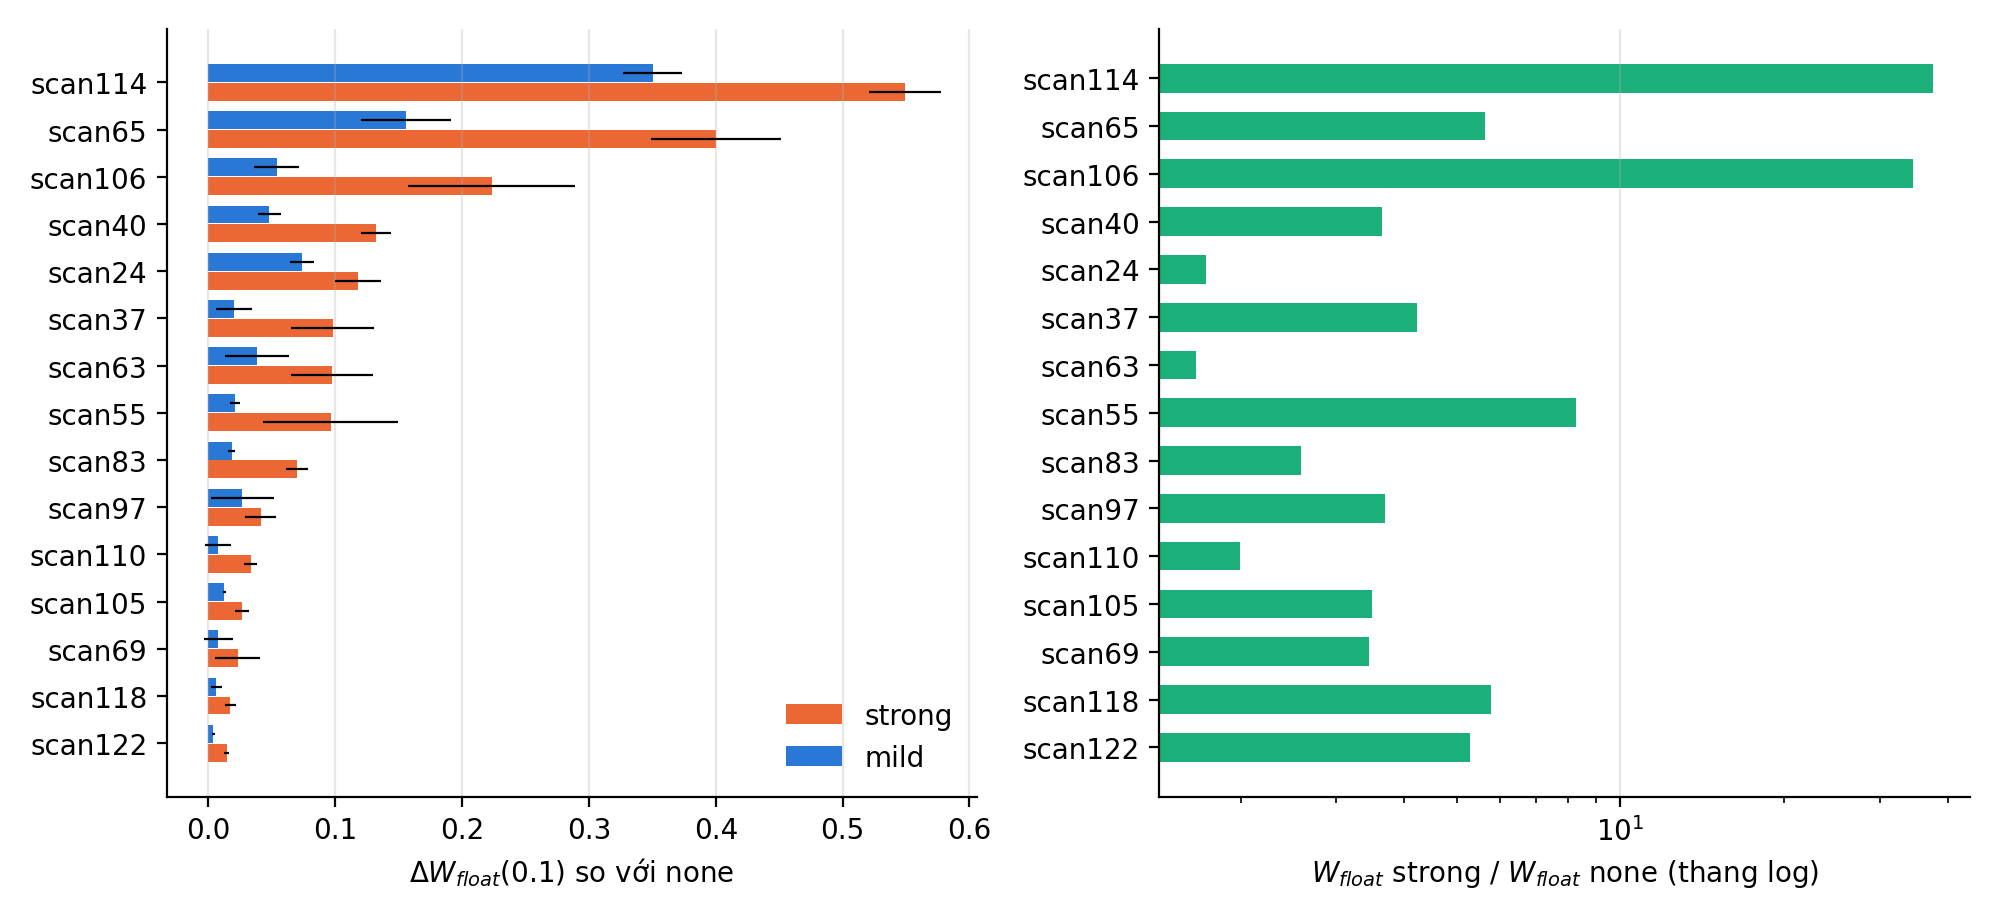
\includegraphics[width=\textwidth]{figures/t2_go.png}
\caption{3DGS chuẩn (SH3, khởi tạo SfM, gsplat, 10k vòng), 3 seed. Trái: $\dW$ mild và strong. Phải: tỉ số $\W$ strong / $\W$ none (thang log).}
\end{figure}
\begin{table}[H]
\centering\small
\caption{3DGS chuẩn, $N=8$, trung bình 3 seed.}
\begin{tabular}{@{}lcccccc@{}}
\toprule
Scan & $\W$ none & $\dW$ mild & $\dW$ strong & up strong & PSNR none & PSNR strong \\
\midrule
scan24 & 0.162 & $+0.074$ & $+0.118$ & 3/3 & 20.58 & 15.39 \\
scan37 & 0.030 & $+0.020$ & $+0.098$ & 3/3 & 20.39 & 16.37 \\
scan40 & 0.050 & $+0.048$ & $+0.132$ & 3/3 & 21.73 & 15.38 \\
scan55 & 0.013 & $+0.021$ & $+0.096$ & 3/3 & 23.96 & 19.11 \\
scan63 & 0.148 & $+0.038$ & $+0.097$ & 3/3 & 26.17 & 21.04 \\
scan65 & 0.087 & $+0.156$ & $+0.400$ & 3/3 & 23.13 & 16.82 \\
scan69 & 0.009 & $+0.008$ & $+0.023$ & 3/3 & 20.09 & 18.57 \\
scan83 & 0.044 & $+0.018$ & $+0.070$ & 3/3 & 26.46 & 23.12 \\
scan97 & 0.015 & $+0.027$ & $+0.041$ & 3/3 & 22.71 & 18.63 \\
scan105 & 0.011 & $+0.013$ & $+0.027$ & 3/3 & 24.79 & 19.49 \\
scan106 & 0.007 & $+0.054$ & $+0.223$ & 3/3 & 21.81 & 17.49 \\
scan110 & 0.033 & $+0.008$ & $+0.033$ & 3/3 & 22.15 & 20.39 \\
scan114 & 0.015 & $+0.350$ & $+0.549$ & 3/3 & 24.20 & 14.36 \\
scan118 & 0.004 & $+0.006$ & $+0.017$ & 3/3 & 24.68 & 20.87 \\
scan122 & 0.003 & $+0.004$ & $+0.014$ & 3/3 & 26.65 & 22.18 \\
\bottomrule
\end{tabular}
\end{table}
\begin{itemize}
  \item $\dW$ strong dương ở \textbf{15/15 scan} (45/45 cặp), trung vị $+0.096$; mild tăng ở 44/45 cặp. Tiêu chí đặt trước (\(\ge80\%\) scan dương và trung vị \(\ge0.03\)) được đáp ứng: \textbf{GO}.
  \item Độ lớn tuyệt đối khác nhau nhiều ($+0.014$ đến $+0.549$). Ở các scan có mức tăng tuyệt đối nhỏ, mức nền rất thấp (0.003--0.015), nên $\W$ strong vẫn gấp 3--6 lần mức none; tỉ số chung 1.7--38 lần.
  \item So với pipeline nghiên cứu, mức tăng nhỏ hơn 2.1--4.6 lần trên 3 scan cũ (scan24 0.118 so với 0.261; scan63 0.097 so với 0.204; scan83 0.070 so với 0.324), nhất quán với E9.
  \item Lưu ý: khởi tạo SfM từ 8 view rất thưa (scan63: 137 điểm); số điểm của các scan khác chưa được kiểm tra. Mật độ hoá hoạt động bình thường (khoảng 50\,000 Gaussian cuối cùng trên scan63).
\end{itemize}

\subsection{E-A: hoán vị cách gán nhiễu và chỉ số xung đột}
\label{sec:ea}
Chỉ số xung đột có trọng số chồng lấn (tính trước khi huấn luyện):
\[ I_{\text{conflict}}=\frac{\sum_{i<j}O_{ij}\,\lVert\log\phi_i(\bar I)-\log\phi_j(\bar I)\rVert^2}{\sum_{i<j}O_{ij}}, \]
với $O_{ij}$ là tỉ lệ điểm bề mặt tham chiếu nhìn thấy được ở cả hai view $i,j$ (trong mặt nạ, qua kiểm tra z-buffer) và $\bar I$ là cường độ trung bình của vật thể. E-A giữ nguyên tập 8 phép biến đổi của cấu hình strong (seed 0), chỉ hoán vị cách gán cho camera; 4 hoán vị được chọn trong $8!$ cách theo $I_{\text{conflict}}$ (nhỏ nhất, phân vị 1/3, 2/3, lớn nhất). Phương sai của nhiễu giữ nguyên tuyệt đối giữa các hoán vị.
\begin{table}[H]
\centering\small
\caption{$I_{\text{conflict}}$ và $\dW$ strong (3 seed; cấu hình gốc E8 seed 0: 5 seed).}
\begin{tabular}{@{}lcccc@{}}
\toprule
& \multicolumn{2}{c}{scan63} & \multicolumn{2}{c}{scan83} \\
\cmidrule(lr){2-3}\cmidrule(lr){4-5}
Cấu hình & $I_{\text{conflict}}$ & $\dW$ & $I_{\text{conflict}}$ & $\dW$ \\
\midrule
Hoán vị min & 1.160 & $+0.131$ & 1.138 & $+0.186$ \\
Hoán vị phân vị 1/3 & 1.476 & $+0.154$ & 1.451 & $+0.195$ \\
Hoán vị phân vị 2/3 & 1.547 & $+0.157$ & 1.520 & $+0.377$ \\
Hoán vị max & 1.723 & $+0.228$ & 1.638 & $+0.262$ \\
E8 seed 0 (gán gốc) & 1.596 & $+0.204$ & 1.481 & $+0.324$ \\
E8 seed 1 & 1.046 & $+0.109$ & 0.701 & $+0.081$ \\
E8 seed 2 & 1.427 & $+0.219$ & 1.381 & $+0.269$ \\
\midrule
Spearman $\rho(I_{\text{conflict}},\dW)$ & \multicolumn{2}{c}{$+0.79$} & \multicolumn{2}{c}{$+0.71$} \\
\bottomrule
\end{tabular}
\end{table}
\begin{figure}[H]
\centering
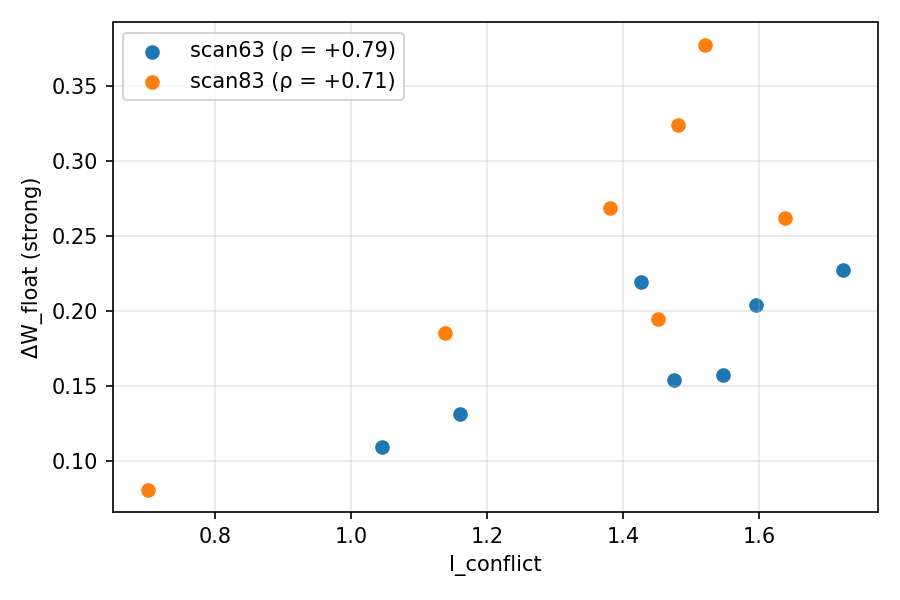
\includegraphics[width=0.6\textwidth]{figures/EA_conflict.png}
\caption{$I_{\text{conflict}}$ và $\dW$ strong cho 7 cấu hình mỗi scan.}
\end{figure}
\interp Với cùng một tập phép biến đổi, chỉ đổi camera nào nhận biến đổi nào làm $\dW$ thay đổi 1.7 lần (scan63) và 2.0 lần (scan83). Đây là bằng chứng can thiệp cho thấy \textbf{cấu trúc xung đột giữa các camera chồng lấn} quyết định độ lớn tác động, và giải thích được biến thiên 3--4 lần của E8. Giới hạn: 7 cấu hình mỗi scan, 2 scan; quan hệ không đơn điệu hoàn toàn (scan83: phân vị 2/3 lớn hơn max).

\subsection{E13: ngoại lệ oracle trên scan83}
\label{sec:e13}
\begin{table}[H]
\centering\small
\caption{$\dW$ strong, $N=8$, khởi tạo ngẫu nhiên (scan63 / scan83).}
\begin{tabular}{@{}lcc@{}}
\toprule
Biến thể & $\dW$ & up \\
\midrule
Gốc (nhiễu có clip) & $+0.204$ / $+0.324$ & 5/5, 5/5 \\
Gốc, nhiễu không clip & $+0.212$ / $+0.348$ & 3/3, 3/3 \\
Oracle, nhiễu có clip & $+0.003$ / $+0.132$ & 2/3, 3/3 \\
Oracle, nhiễu không clip & $-0.011$ / $+0.115$ & 1/3, 3/3 \\
Oracle + mặt nạ bão hoà & $+0.026$ / $+0.063$ & 3/3, 3/3 \\
Oracle, khởi tạo visual hull (E12) & $-0.006$ / $+0.001$ & 0/3, 2/3 \\
\bottomrule
\end{tabular}
\end{table}
\interp Bỏ phép clip không làm biến mất phần còn lại trên scan83 ($+0.115$); mặt nạ bão hoà giảm một nửa. Với visual hull, oracle xoá hết. Giả thuyết ``ngoại lệ do mất thông tin ở vùng bão hoà'' \textbf{không được ủng hộ} là nguyên nhân chính; phần còn lại gắn với khởi tạo ngẫu nhiên (Gaussian khởi tạo ngoài vật thể).

\subsection{M2: GC-ILA (căn chỉnh dạng đóng có ràng buộc gauge)}
\label{sec:gc}
Tại mỗi vòng lặp, với ảnh huấn luyện $k$ và kênh $c$: giải bình phương tối thiểu có trọng số trong miền log cường độ $\log I'_{k,c}\approx a_{k,c}\log\hat I_{k,c}+b_{k,c}$ trên pixel vật thể không bão hoà (cường độ trong $(0.02, 0.98)$), có chính quy hoá kéo $a$ về 1; làm mượt bằng trung bình trượt ($\eta=0.2$); chiếu lên ràng buộc gauge $\prod_k a_{k,c}=1$, $\sum_k b_{k,c}=0$; áp lên ảnh kết xuất không lan truyền gradient qua hệ số; loại pixel bão hoà khỏi hàm mất mát.
\begin{table}[H]
\centering\small
\caption{GC-ILA so với các biến thể khác (scan63 / scan83).}
\begin{tabular}{@{}lcccc@{}}
\toprule
Cấu hình & $\W$ none & $\dW$ strong & PSNR trực tiếp strong & PSNR trực tiếp none \\
\midrule
\multicolumn{5}{@{}l}{\emph{Khởi tạo ngẫu nhiên}} \\
Gốc & 0.262 / 0.162 & $+0.204$ / $+0.324$ & 19.41 / 21.08 & 24.24 / 25.97 \\
M1 (không gauge) & 0.311 / 0.193 & $+0.033$ / $+0.032$ & 12.33 / 12.71 & 12.14 / 12.51 \\
GC-ILA & 0.249 / 0.212 & $+0.006$ / $+0.185$ & 23.58 / 24.99 & 23.22 / 25.49 \\
\midrule
\multicolumn{5}{@{}l}{\emph{Khởi tạo visual hull (E12)}} \\
Gốc & 0.280 / 0.080 & $+0.083$ / $+0.068$ & 19.54 / 22.88 & 23.72 / 26.06 \\
Affine học lr $10^{-2}$ & 0.266 / 0.078 & $+0.072$ / $+0.030$ & 21.28 / 23.29 & 23.24 / 25.65 \\
GC-ILA & 0.274 / 0.079 & $-0.001$ / $+0.005$ & 22.90 / 25.30 & 22.64 / 25.62 \\
Oracle & -- & $-0.006$ / $+0.001$ & 23.50 / 25.95 & -- \\
\bottomrule
\end{tabular}
\end{table}
\interp (i) Ràng buộc gauge khắc phục lỗi mất màu của M1: PSNR trực tiếp từ khoảng 12 dB lên 23--25 dB, cao hơn cấu hình gốc 2.4--4.2 dB khi có nhiễu. (ii) Với visual hull, GC-ILA xoá mức tăng ngang oracle trên cả hai scan, trong khi affine học vẫn giữ 44--87\%. (iii) Với khởi tạo ngẫu nhiên, scan83 còn $+0.185$ (57\% mức gốc), cùng hiện tượng với oracle (Mục~\ref{sec:e13}). (iv) Chi phí trên ảnh sạch: PSNR trực tiếp mức none thấp hơn gốc 0.4--1.1 dB. Tiêu chí đặt trước cho khởi tạo ngẫu nhiên (tỉ lệ $\le0.3$ trên cả hai scan) chưa đạt vì scan83.

\subsection{E12: thời điểm bù và quỹ đạo huấn luyện}
\label{sec:e12}
Khởi tạo visual hull, lưu snapshot ở các vòng 250--5000. ``warm-up'': 1000 vòng đầu đóng băng vị trí, kích thước, hướng của Gaussian và tắt mật độ hoá (độ mờ, màu và mô-đun bù vẫn học).
\begin{table}[H]
\centering\small
\caption{$\dW$ strong cuối huấn luyện (scan63 / scan83).}
\begin{tabular}{@{}lcc@{}}
\toprule
Lịch huấn luyện & Không bù & Affine học lr $10^{-2}$ \\
\midrule
Đồng thời & $+0.083$ / $+0.068$ & $+0.072$ / $+0.030$ \\
Warm-up 1000 vòng & $+0.108$ / $+0.092$ & $+0.075$ / $+0.029$ \\
\bottomrule
\end{tabular}
\end{table}
\begin{figure}[H]
\centering
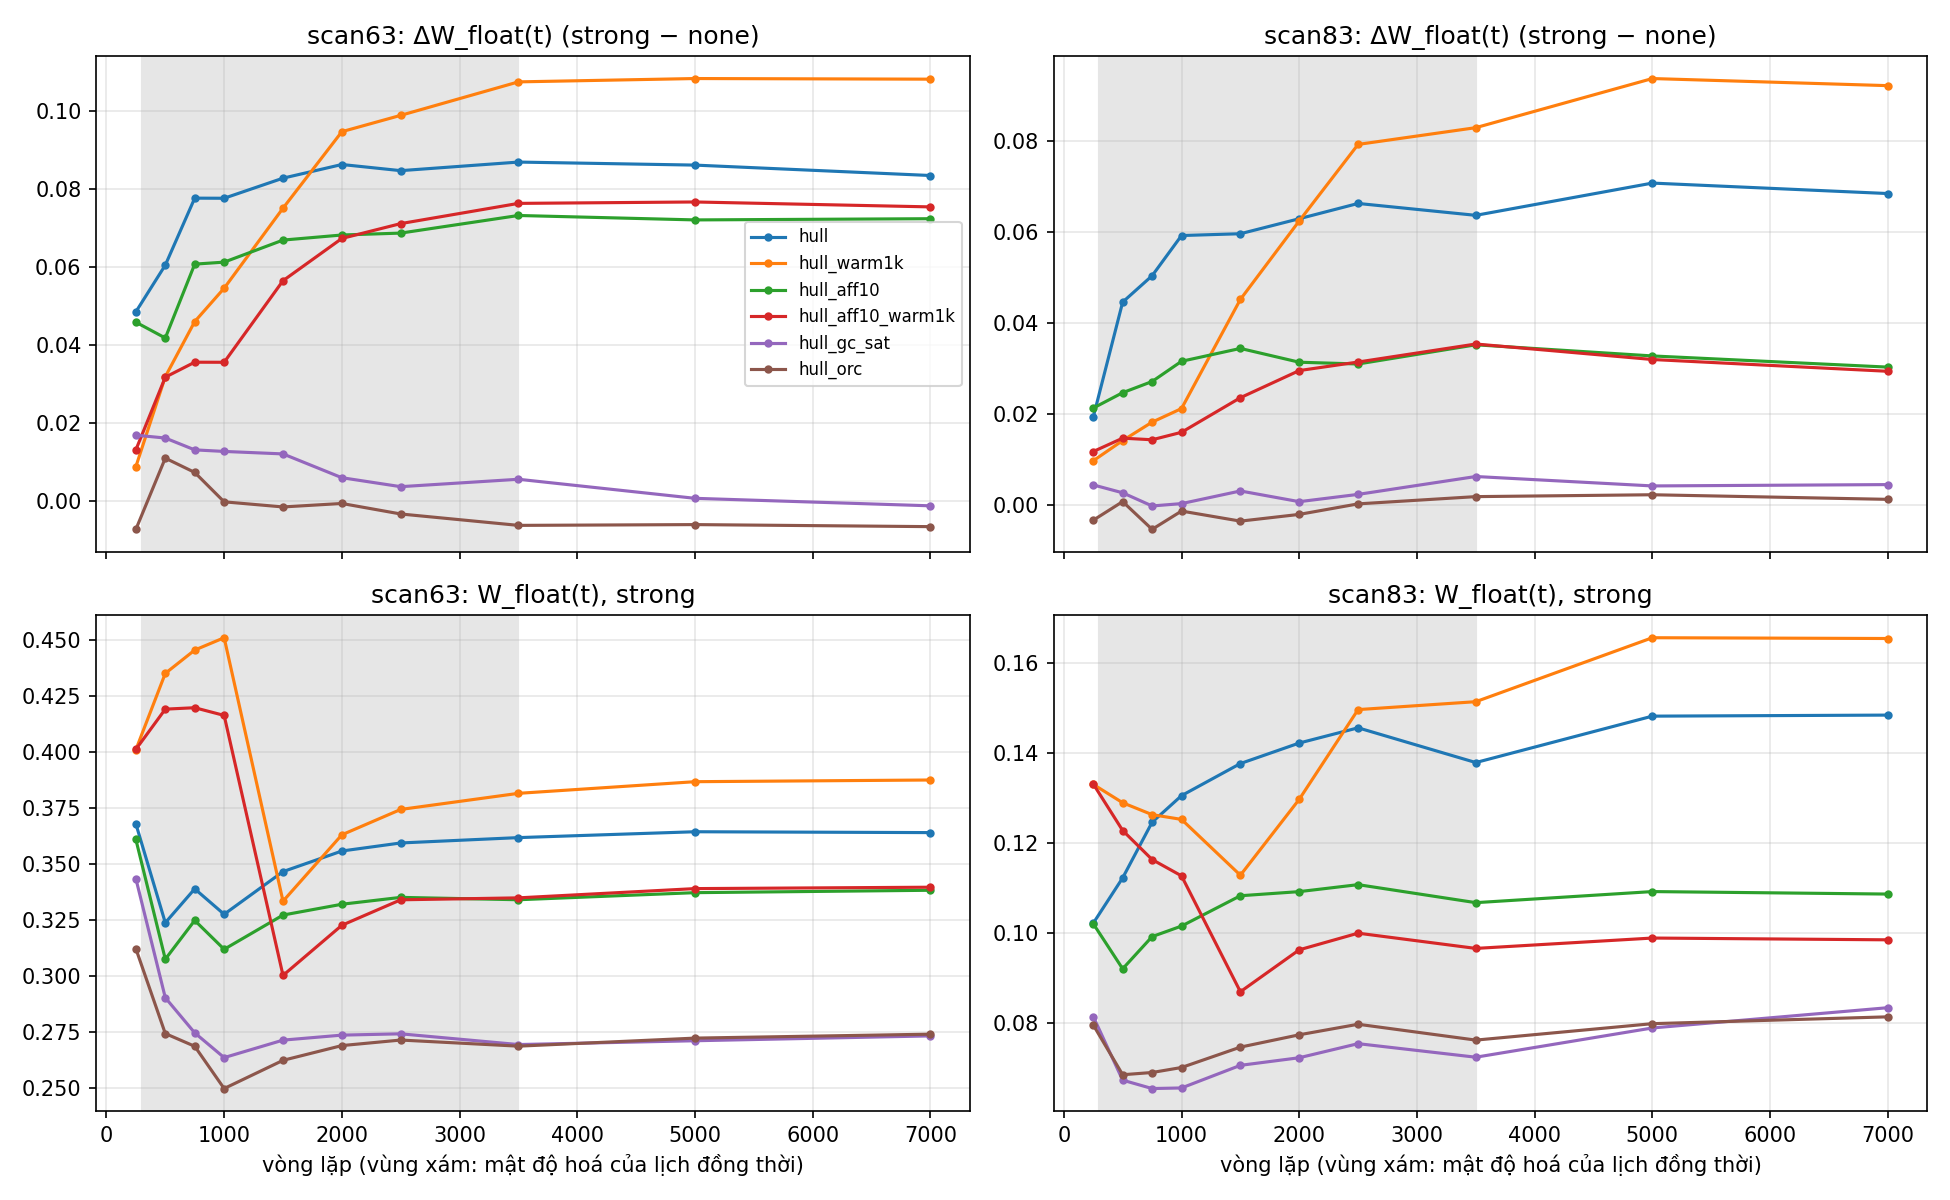
\includegraphics[width=\textwidth]{figures/E12_trajectories.png}
\caption{Trên: $\dW(t)$; dưới: $\W(t)$ ở mức strong. Vùng xám: mật độ hoá của lịch đồng thời. Snapshot ở vòng 3000 (ngay sau khi đặt lại độ mờ) được bỏ.}
\end{figure}
\interp (i) Warm-up không giảm floater của affine học ($-4\%$ / $+3\%$), còn làm tăng floater khi không có bù ($+30\%$ / $+35\%$): giả thuyết ``bù học chậm hơn mật độ hoá'' \textbf{không được ủng hộ} ở dạng đã kiểm tra. (ii) $\dW$ đã khoảng 0.05 ở vòng 250, trước khi mật độ hoá bắt đầu (vòng 300). (iii) Trong 1000 vòng đóng băng hình học, $\W$ mức strong vẫn tăng (scan63: 0.40 $\to$ 0.45): sai lệch được giải thích bằng cách tăng độ mờ của các Gaussian có sẵn ngoài bề mặt. Như vậy sai lệch rò vào hình học từ rất sớm và không chỉ qua mật độ hoá. (iv) GC-ILA và oracle giữ $\dW(t)\approx0$ suốt quá trình. Nguyên nhân affine học thất bại chưa được xác định; chưa đo sai số tham số affine theo thời gian.

\subsection{Chỉ số có xét hình dạng Gaussian}
\label{sec:wsig}
$\W^\Sigma$: thay chỉ báo $d_i>\tau$ bằng tỉ lệ trong 7 điểm (tâm và $\pm1\sigma$ dọc 3 trục chính của Gaussian) cách bề mặt hơn $\tau$. Trên toàn bộ checkpoint, tương quan giữa $\W$ và $\W^\Sigma$ là 0.999, và mọi bảng $\dW$ cho cùng kết luận khi dùng $\W^\Sigma$. Chỉ số khoảng cách tâm không làm sai lệch kết luận.

%=====================================================================
\section{Tổng hợp trạng thái giả thuyết}
\label{sec:status}
\begin{table}[H]
\centering\small
\begin{tabularx}{\textwidth}{@{}p{4.6cm} Y p{2.9cm}@{}}
\toprule
Giả thuyết & Bằng chứng chính & Trạng thái \\
\midrule
P1: floater tăng theo $S$ & 26/26 cặp (pipeline nghiên cứu); 45/45 cặp, 15/15 scan (3DGS chuẩn); vững với SH3, cắt kích thước, bù affine, visual hull, $\tau$, $\W^\Sigma$ & \ok \\
P2: tác động lớn hơn khi $N$ nhỏ & $\hat\beta_{NS}\approx0$ trên $N=4$--16 & \no \\
P3: floater phía trước bề mặt & front(0.1) tăng 15/18 cặp; khoảng cách tới camera giảm ít & \partly \\
P4: cải thiện ảnh $\neq$ cải thiện hình học & Affine học: PSNR tăng, floater giảm ít; M1: ngược lại & \ok \\
Floater riêng cho 1--2 view, sát camera & Floater được nhiều view quan sát; khoảng cách tới camera giảm 4--8\% & \no \\
Nguyên nhân là sự khác nhau giữa các ảnh & Biến đổi chung, nhiễu theo pixel: $\dW\approx0$ & \ok \\
Thành phần $\gamma$ là cần thiết & Không $\gamma$ giữ 83--99\% & \no \\
Thiếu dung lượng màu & SH3 giữ 61--100\%; affine thất bại cả khi đúng lớp mô hình & \no \\
Cấu trúc gán nhiễu quyết định độ lớn & Hoán vị: $\times1.7$--$2.0$; $\rho=+0.79$, $+0.71$ & \ok{} (2 scan) \\
Bù học chậm hơn mật độ hoá & Warm-up không giúp & \no \\
Ngoại lệ oracle do clip bão hoà & Không clip vẫn $+0.115$; hull: $+0.001$ & \no \\
Bù khớp đúng tại mỗi bước loại floater & Oracle, GC-ILA với hull: $\dW\approx0$ & \ok{} (khởi tạo tốt) \\
Khởi tạo ngẫu nhiên khuếch đại & Hull: còn 16--59\%; 3DGS chuẩn nhỏ hơn 2.1--4.6 lần & \ok \\
Bất đồng giữa mô hình kém tin cậy khi có sai lệch & AUROC 0.84--0.89, tăng theo $S$ & \no \\
\bottomrule
\end{tabularx}
\end{table}

%=====================================================================
\section{Diễn giải tổng thể}
\begin{enumerate}
  \item \textbf{Điều kiện xuất hiện.} Floater xuất hiện khi các camera cùng quan sát một vùng nhận các phép biến đổi trắc quang khác nhau. Một biến đổi chung được hấp thụ vào màu; nhiễu không có cấu trúc theo ảnh được trung bình hoá. Độ lớn phụ thuộc vào cấu trúc xung đột trên đồ thị đồng quan sát của camera ($I_{\text{conflict}}$), không chỉ vào biên độ nhiễu.
  \item \textbf{Cơ chế.} Khi không tồn tại một trường màu nhất quán giải thích mọi ảnh, phần dư được giảm bằng hình học: các Gaussian ngoài bề mặt (có sẵn từ khởi tạo hoặc sinh ra khi mật độ hoá) được tăng độ mờ và che bề mặt một cách khác nhau ở từng view (thị sai). Quá trình bắt đầu ngay từ những vòng lặp đầu. Khởi tạo có nhiều Gaussian ngoài vật thể khuếch đại hiện tượng.
  \item \textbf{Vì sao bù ngoại hình học được không đủ.} SH bậc 3 và affine học có đủ bậc tự do nhưng vẫn để lọt phần lớn floater; khởi động trước không giúp. Ngược lại, phép bù khớp đúng tại mỗi bước (oracle, GC-ILA) xoá được hiệu ứng khi khởi tạo tốt. Giả thuyết còn mở: affine học không hội tụ tới đúng phép biến đổi (mơ hồ giữa màu cảnh và hệ số theo ảnh), trong khi GC-ILA được cố định gauge và giải đúng nghiệm tại mỗi bước.
  \item \textbf{Số góc nhìn.} Không có tương tác nhất quán; tăng $N$ tới 16 không tự loại bỏ tác động.
\end{enumerate}

%=====================================================================
\section{Giới hạn và việc tiếp theo}
\paragraph{Giới hạn.}
\begin{itemize}
  \item Chỉ DTU và nhiễu ISP tổng hợp toàn ảnh; chưa có dữ liệu thực có auto-exposure, chưa xét thay đổi chiếu sáng vật lý (bóng đổ, phản xạ).
  \item Các thí nghiệm cơ chế (E1--E13, E-A, GC-ILA) chủ yếu trên scan63, scan83 với pipeline nghiên cứu; chưa chạy trên 3DGS chuẩn 15 scan.
  \item Khởi tạo SfM của T2 rất thưa; chưa kiểm tra số điểm của các scan.
  \item Chưa so sánh với các phương pháp khác (baseline).
\end{itemize}
\paragraph{Kế hoạch v3 (đề xuất).}
\begin{enumerate}
  \item GC-ILA và affine học trên 3DGS chuẩn, 15 scan (bảng kết quả chính).
  \item Chẩn đoán affine học: sai số tham số theo thời gian; GC-ILA cố định hệ số sau 1000 vòng.
  \item E-A trên 3DGS chuẩn với nhiều scan hơn, ước lượng quan hệ $I_{\text{conflict}}$--$\dW$ có khoảng tin cậy.
  \item Dữ liệu thực có auto-exposure (bộ dữ liệu của Gaussian-DK); trộn 7 điều kiện chiếu sáng của DTU.
  \item Baseline: WildGaussians, Luminance-GS, HarmoGS, FastWild-GS, CoR-GS.
\end{enumerate}

%=====================================================================
\appendix
\section{Vị trí dữ liệu và mã nguồn}
\sloppy
\begin{itemize}
  \item Kết quả pha 1: \texttt{results/final/} (\texttt{final\_with\_delta.csv}, \texttt{E7\_signals.csv}).
  \item Kết quả v2: \texttt{results/v2/} (\texttt{v2\_with\_delta.csv}, \texttt{v2\_snaps.csv}, \texttt{old\_v2eval.csv}, \texttt{EA\_perms.json}).
  \item Notebook: \texttt{notebooks/colab\_rq1\_final.ipynb} (pha 1), \texttt{notebooks/colab\_v2\_mechanism.ipynb} (v2).
  \item Đánh giá: \texttt{scripts/floater\_metrics.py}, \texttt{scripts/fm2.py}; khởi tạo SfM: \texttt{scripts/sfm\_tri.py}.
  \item Quy ước tên run v2: \texttt{runs/v2\_<mức><tags>\_dtu\_scan<s>\_v<N>}; tags: \texttt{\_hull}, \texttt{\_aff10}, \texttt{\_gc}, \texttt{\_orc}, \texttt{\_sat}, \texttt{\_noclip}, \texttt{\_warm1k}, \texttt{\_p<min|lo|hi|max>}, \texttt{\_std}.
\end{itemize}

\end{document}
